\documentclass[]{standalone}

\begin{document}
	\begin{frame}{Reults}{\textbf{Pre}-Processing}
	\vspace{-25pt}
	Dice coefficient measures overlapping between two images.
	\begin{columns}
		\begin{column}{0.45\textwidth}
		\begin{figure}[h!]
		\footnotesize
		\centering
			\begin{subfigure}[h!]{0.49\textwidth}
			\hfill
			     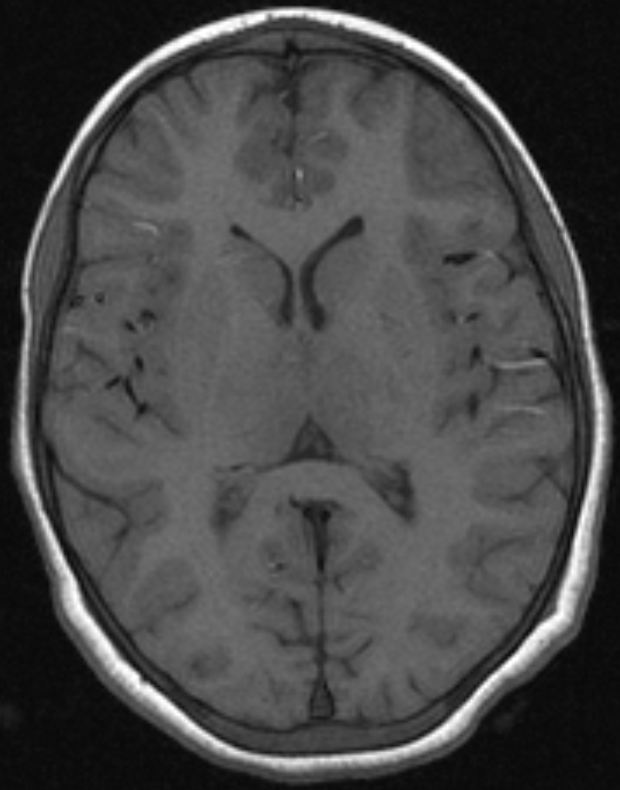
\includegraphics[scale=0.11]{./IMG/T1W0.png}
			     \caption*{Original Scan} 
			\end{subfigure}
			\hfill
			\begin{subfigure}[h!]{0.49\textwidth}
			     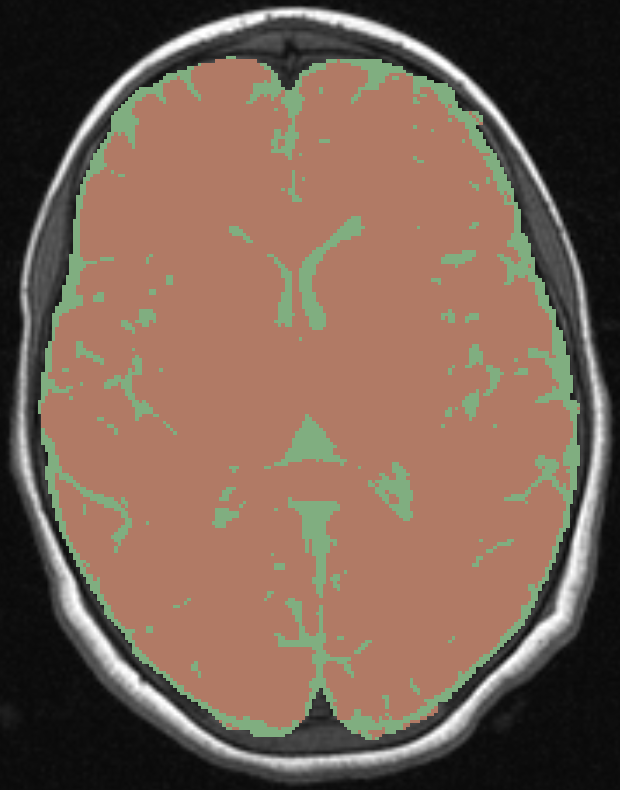
\includegraphics[scale=0.11]{./IMG/SEG0.png}
			     \caption*{Segmentation}
			\end{subfigure}
			\caption*{Pipeline Fault}
		\end{figure}
		\end{column}
		
		\begin{column}{0.55\textwidth}
			\begin{figure}[h!]
			\footnotesize
			\centering
				\begin{subfigure}[h!]{0.32\textwidth}
				     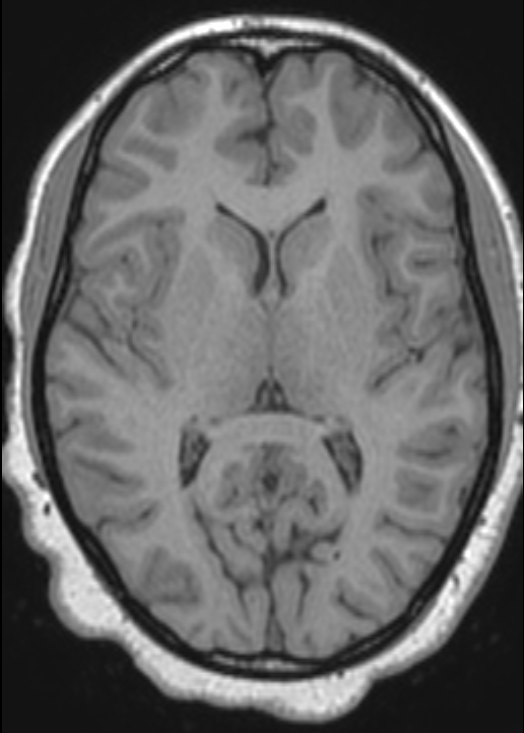
\includegraphics[scale=0.1085]{./IMG/T1W54_2.png}
				     \caption*{Original Scan} 
				\end{subfigure}
				\hfill
				\begin{subfigure}[h!]{0.32\textwidth}
				     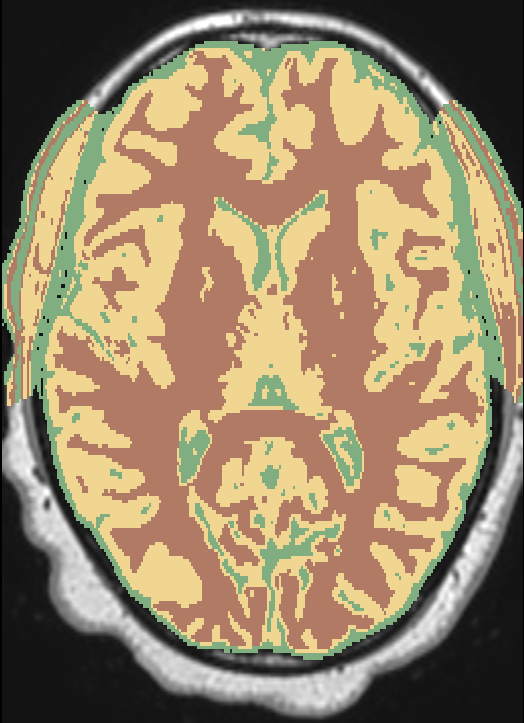
\includegraphics[scale=0.11]{./IMG/FSL_SEG54.png}
				     \caption*{FSL}
				\end{subfigure}
				\hfill
				\begin{subfigure}[h!]{0.32\textwidth}
				     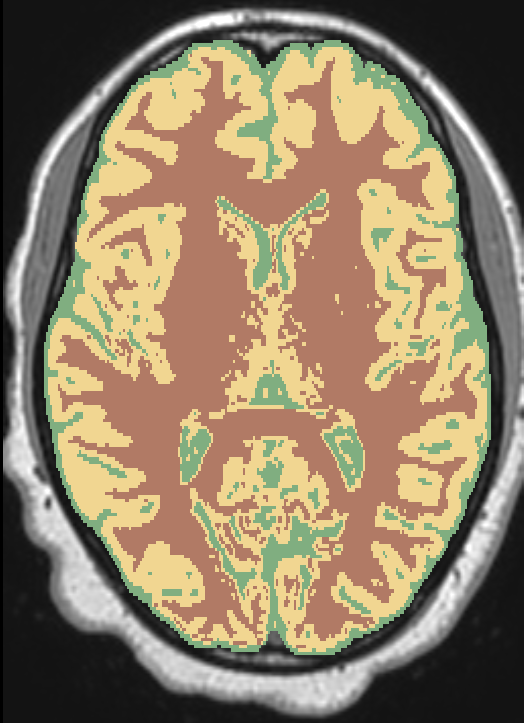
\includegraphics[scale=0.11]{./IMG/SEG54.png}
				     \caption*{Pipeline}
				\end{subfigure}
				\caption*{FSL Fault}
			\end{figure}
		\end{column}
	\end{columns}
	\end{frame}
\end{document}
